\begin{figure}[htb]
    \centering
    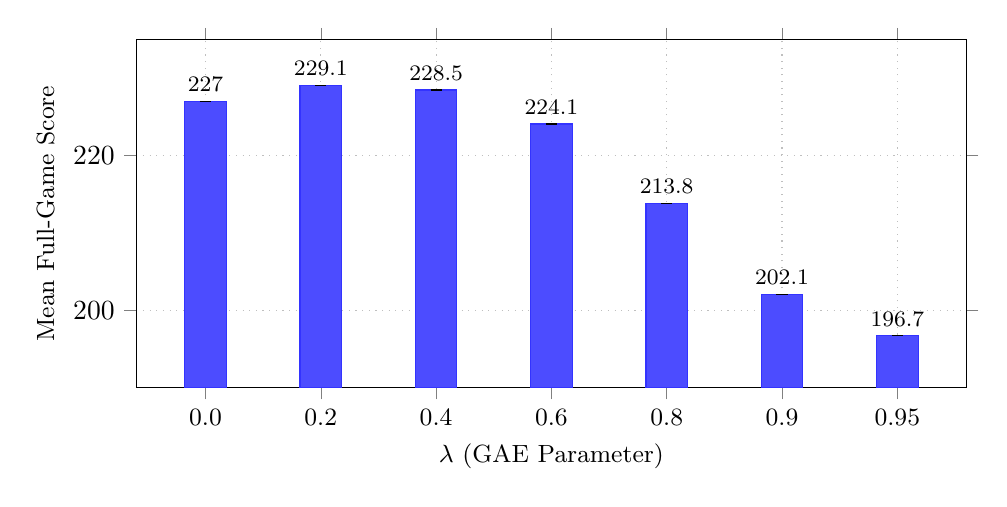
\begin{tikzpicture}
        \begin{axis}[
                ybar,
                width=\columnwidth,
                height=6cm,
                xlabel={$\lambda$ (GAE Parameter)},
                ylabel={Mean Full-Game Score},
                symbolic x coords={0.0, 0.2, 0.4, 0.6, 0.8, 0.9, 0.95},
                xtick=data,
                xticklabel style={font=\small},
                ylabel style={font=\small},
                xlabel style={font=\small},
                bar width=15pt,
                ymin=190, ymax=235,
                grid=both,
                grid style={dotted},
                tick align=outside,
                nodes near coords,
                nodes near coords style={font=\footnotesize, anchor=south},
            ]

            \addplot[
                fill=blue!70!white,
                draw=blue!80!white,
                error bars/.cd,
                y dir=both,
                y explicit
            ] coordinates {
                    (0.0, 227.0) +- (0, 0)
                    (0.2, 229.1) +- (0, 0)
                    (0.4, 228.5) +- (0, 0)
                    (0.6, 224.1) +- (0, 0)
                    (0.8, 213.8) +- (0, 0)
                    (0.9, 202.1) +- (0, 0)
                    (0.95, 196.7) +- (0, 0)
                };

        \end{axis}
    \end{tikzpicture}
    \caption{Final performance by GAE lambda}
    \label{fig:gae-lambda-performance}
\end{figure}